
% This LaTeX was auto-generated from an M-file by MATLAB.
% To make changes, update the M-file and republish this document.

\documentclass{article}
\usepackage{graphicx}
\usepackage{color}

\sloppy
\definecolor{lightgray}{gray}{0.5}
\setlength{\parindent}{0pt}

\begin{document}

    
    \begin{verbatim}
close all;
clear all;
load('fisheriris');
[r, c]=size(meas);
% Extend meas by 1 to account for the bias
col1 = ones(r,1);
emeas=[col1 meas];

%Assign numerical labels
for i=1:50, class(i)=1; end %setosa
for i=51:100, class(i)=2; end %versicolor
for i = 101:150, class(i) = 3; end %virginica
%Transform numerical lables into 0 / 1 labels
newclass(class==1) = 0; %setosa becomes class 0%
% the rest are in class 1
newclass(class == 2) = 1;
newclass(class == 3) = 1;
p = 0.1; % extent of training sets
randindex=randperm(r);
N = round(p*r)
train = emeas(randindex(1:N),:);
trainlabels = newclass(randindex(1:N));
test = emeas(randindex(N+1:r),:);
testlabels = newclass(randindex(N+1:r));
%N = 15;

% initialize w
w=zeros(c+1,1);
w2=zeros(c+1,1);
ybar=mean(trainlabels);
w(1)=log(ybar/(1-ybar));
s=zeros(1,N);
z=zeros(N,1);

%Convergence Criterion
epsil = 2.2204e-16;
iter = 100000;
s0 = 0;

%Alg 8.2

%Signmoid function

%mui = exp(mu) / (exp(mu) + 1);


for i = 1:iter,

    eta = w(1) + train * w;
    mu = exp(eta) ./ (exp(eta) + 1);
    s = mu.*(1-mu);
    z = eta + (trainlabels'-mu) ./ s;
    S = diag(s);

    fprintf('The value of s is %d.\n',s(1))
    fprintf('The iteration number is %d.\n',i)

    %Calculate the difference between previous and current s
    sDiff = S(1) - s0;
    if (sDiff < epsil),
        fprintf('The value of s is %d.\n',s(1))
        fprintf('Converged in %d steps\n',i)
        break;
    end

    s0 = S(1);
    w = inv(train'*S*train)*train'*S*z;

end


%Test

ltest=length(testlabels);
% Compute the output for each test data using w
for i=1:ltest,
out(i)=test(i,:)*w;
end
% Transform output in 0 1 labels
out1=out;
out1(out<0)=0;
out1(out>0)=1;
% compute accuracy
accuracy = 1 - sum(abs(testlabels - out1))/ltest
%plot ROC curves
figure
plotroc(testlabels, out1);
% plot confusion matrix
figure
plotconfusion(testlabels, out1);
\end{verbatim}

        \color{lightgray} \begin{verbatim}
N =

    15

The value of s is 2.455948e-01.
The iteration number is 1.
The value of s is 5.355942e-02.
The iteration number is 2.
The value of s is 5.355942e-02.
Converged in 2 steps

accuracy =

     1

\end{verbatim} \color{black}
    
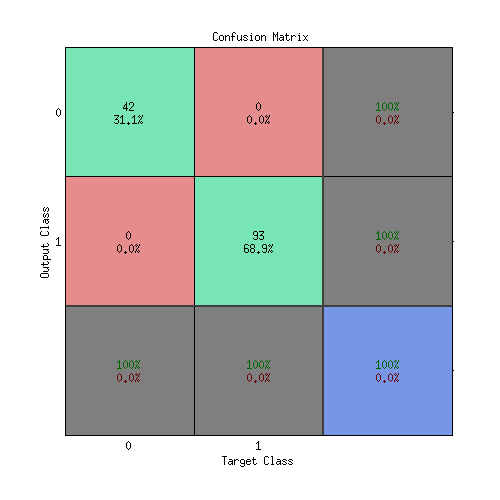
\includegraphics [width=4in]{VersicolorVsVirginicaAndSetosa_ConfusionMatrix.png}

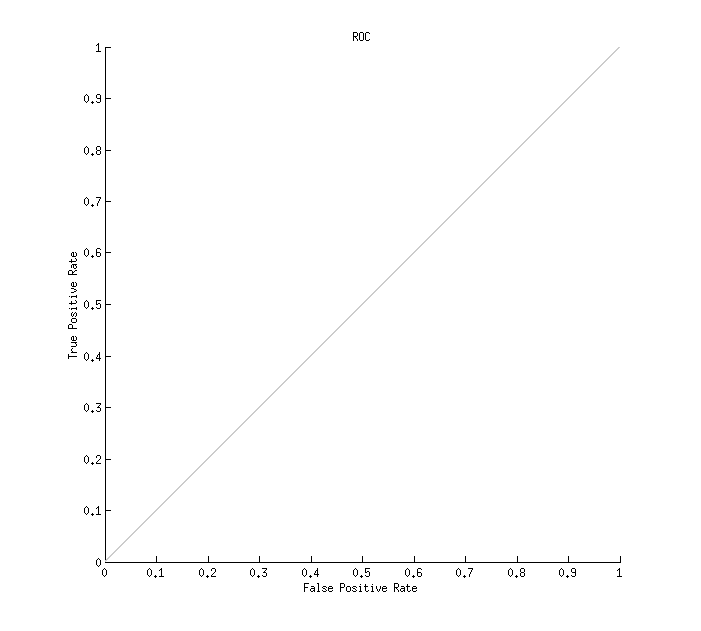
\includegraphics [width=4in]{VersicolorVsVirginicaAndSetosa_ROC.png}



\end{document}
    
